%%%%%%%%%%%%%%%%%%%%%%%%%%%%%%%%%%%%%%%%%
% Jacobs Landscape Poster
% LaTeX Template
% Version 1.0 (29/03/13)
%
% Created by:
% Computational Physics and Biophysics Group, Jacobs University
% https://teamwork.jacobs-university.de:8443/confluence/display/CoPandBiG/LaTeX+Poster
% 
% Further modified by:
% Nathaniel Johnston (nathaniel@njohnston.ca)
%
% This template has been downloaded from:
% http://www.LaTeXTemplates.com
%
% License:
% CC BY-NC-SA 3.0 (http://creativecommons.org/licenses/by-nc-sa/3.0/)
%
%%%%%%%%%%%%%%%%%%%%%%%%%%%%%%%%%%%%%%%%%

%----------------------------------------------------------------------------------------
%	PACKAGES AND OTHER DOCUMENT CONFIGURATIONS
%----------------------------------------------------------------------------------------

\documentclass[landscape,a0paper,fontscale=0.285]{beamer} % Adjust the font scale/size here

\usepackage[scale=1.24]{beamerposter} % Use the beamerposter package for laying out the poster

\usetheme{confposter} % Use the confposter theme supplied with this template

\setbeamercolor{block title}{fg=nblue,bg=white} % Colors of the block titles
\setbeamercolor{block body}{fg=black,bg=white} % Colors of the body of blocks
\setbeamercolor{block alerted title}{fg=white,bg=dblue!70} % Colors of the highlighted block titles
\setbeamercolor{block alerted body}{fg=black,bg=dblue!10} % Colors of the body of highlighted blocks
% Many more colors are available for use in beamerthemeconfposter.sty
\usepackage{gensymb} % this is for the degreetemp 

%-----------------------------------------------------------
% Define the column widths and overall poster size
% To set effective sepwid, onecolwid and twocolwid values, first choose how many columns you want and how much separation you want between columns
% In this template, the separation width chosen is 0.024 of the paper width and a 4-column layout
% onecolwid should therefore be (1-(# of columns+1)*sepwid)/# of columns e.g. (1-(4+1)*0.024)/4 = 0.22
% Set twocolwid to be (2*onecolwid)+sepwid = 0.464
% Set threecolwid to be (3*onecolwid)+2*sepwid = 0.708

\newlength{\sepwid}
\newlength{\onecolwid}
\newlength{\twocolwid}
\newlength{\threecolwid}
\setlength{\paperwidth}{60in} % A0 width: 46.8in
\setlength{\paperheight}{36in} % A0 height: 33.1in
\setlength{\sepwid}{0.024\paperwidth} % Separation width (white space) between columns
\setlength{\onecolwid}{0.22\paperwidth} % Width of one column
\setlength{\twocolwid}{0.464\paperwidth} % Width of two columns
\setlength{\threecolwid}{0.708\paperwidth} % Width of three columns
\setlength{\topmargin}{-0.5in} % Reduce the top margin size
%-----------------------------------------------------------

\usepackage{graphicx}  % Required for including images

\usepackage{booktabs} % Top and bottom rules for tables

%----------------------------------------------------------------------------------------
%	TITLE SECTION 
%----------------------------------------------------------------------------------------
\title{Bayesian Analysis of Thrombopoietin (TPO) Levels in Immune Thrombocytopaenia (ITP)} % Poster title

%\author{George Adams, Adam Gosztolai, Anwar A. Sayed, Amna Malik, Elisa Lucchini and Nichola Cooper} % Author(s)

%\institute{Department of Haematology, Imperial College London}% Institution(s)
\author[shortname]{George Adams,  Adam Gosztolai, Anwar A. Sayed, Amna Malik, Elisa Lucchini and Nichola Cooper}
\institute[shortinst]{Centre of Haematology, Department of Medicine, Imperial College London, United Kingdom}


%----------------------------------------------------------------------------------------

\begin{document}
\addtobeamertemplate{headline}{} 
{\begin{tikzpicture}[remember picture, overlay]
     \node [anchor=north west, inner sep=3cm]  at (current page.north west)
     {
\includegraphics[height=5cm]{ic_logo}};
  \end{tikzpicture}}

%----------------------------------------------------------------------------------------
%	TITLE SECTION 
%--------------------------------------------------------------

\addtobeamertemplate{block end}{}{\vspace*{1ex}} % White space under blocks
\addtobeamertemplate{block alerted end}{}{\vspace*{1ex}} % White space under highlighted (alert) blocks

\setlength{\belowcaptionskip}{1ex} % White space under figures
\setlength\belowdisplayshortskip{1ex} % White space under equations

\begin{frame}[t] % The whole poster is enclosed in one beamer frame

\begin{columns}[t] % The whole poster consists of three major columns, the second of which is split into two columns twice - the [t] option aligns each column's content to the top

\begin{column}{\sepwid}\end{column} % Empty spacer column

\begin{column}{\onecolwid} % The first column

%----------------------------------------------------------------------------------------
%	OBJECTIVES
%----------------------------------------------------------------------------------------

%\begin{alertblock}{Summary}

%\begin{itemize}
%    \item The aim of this study was to accurately characterise the relationship between TPO and platelet counts in patients with chronic ITP. 
%    \item A Bayesian regression model was used to determine this relationship as this approach is generally more accurate than traditional methods.
%    \item We demonstrate a non-linear relationship which flattens off at a platelet of approximately 50$\times 10^9/L$. These findings indicate the effect of platelet count itself is relatively small as it influences the TPO levels only at very low platelet counts. 
%\end{itemize}


%\end{alertblock}

%----------------------------------------------------------------------------------------
%	INTRODUCTION
%----------------------------------------------------------------------------------------

\begin{alertblock}{Background}

\paragraph{} Thrombopoietin (TPO) is a growth factor which promotes differentiation and maturation of megakaryocytes and the production of platelets.
In ITP, TPO levels are inappropriately low. The most popular explanation for this is that TPO is \emph{sponged} by binding to platelets which are then removed from the circulation\cite{Kuterreciprocalrelationshipthrombopoietin1995}. However, megakaryocytes are also capable of binding TPO and there it is suggested that the low TPO levels in ITP are chiefly due to an increased megakaryocyte mass\cite{SatoBindingregulationthrombopoietin1998}. This study aims to clarify the relationship between TPO levels and platelet counts in ITP using aplastic anaemia (bone marrow failure) as a comparison. In this study we use a bayesian regression model which unlike traditional regression models does not require a predetermined algorithm but rather infers probability distributions by iterative re-sampling of the data\cite{ChaturvediRobustBayesiananalysis1996}. 

%The physiological processes that regulate the circulating levels of TPO are widely debated and it would seem that  

%In patients with ITP, TPO levels are inappropriately low. The exact reasons for this are not well understood. The predominant hypothesis is that higher rates of platelet turnover in active ITP leads to increased consumption of TPO through binding to high-affinity receptors on the platelet (and megakaryocyte) membrane (the \emph{sponge theory}). To better understand TPO and platelets in ITP, we measured TPO levels in 67 patients with chronic ITP with a range of platelet counts.  We also measured TPO levels in 5 patients with aplastic anaemia as these patients are thrombocytopenic but lack a direct immune-mediated platelet destruction. We analysed the association between TPO and platelet levels using a Bayesian regression model, which is more accurate with smaller sample sizes than classical Gaussian regression models. We use this approach to infer the probability distribution of TPO over a range of different platelet counts. 






\end{alertblock}

\begin{block}{Study Population}

\paragraph{} 67 patients were recruited for this study from our center with a diagnosis of chronic ITP during May to November 2014. 5 Patients were recruited with aplastic anaemia. Each participant had repeated measurements taken over the course of 6 months.  



\end{block}

\begin{block}{Methods}
\paragraph{}Blood samples were collected in duplicate in sodium citrate vacutainer tubes, double spun and stored at -80\textdegree C within four hours of collection. TPO levels were measured using quantitative sandwich ELISA technique.
\paragraph{} We used log-normalised TPO and platelet counts in a bayesian regression model;
\begin{align}
    \log(TPO) \thicksim \text{Norm}(\mu, \sigma) \\
    \mu = \alpha + \beta\times \log(platelet) \\
    \alpha \thicksim\ \text{Norm}(0.01, 10) \\
    \beta \thicksim\ \text{Norm}(0.01, 10) \\
    \sigma \thicksim \text{Uniform}(-1, 1)
\end{align}
\paragraph{} We used uninformative priors for the model (\textit{equation 3, 4, 5}). Posterior distributions were derived using Markov-chain methods with gibbs sampling from 100,000 iterations of the data. \textbf{\textit{Maximium a posteriori} (MAP)} estimates and 90\% Bayesian Confidence intervals (BCI) were calculated platelet counts ranging 1 to 200$x10^9/L$. 
\end{block}
%------------------------------------------------

%\begin{figure}
%
\includegraphics[width=0.8\linewidth]{placeholder.jpg}
%\caption{Figure caption}
%\end{figure}

%----------------------------------------------------------------------------------------

\end{column} % End of the first column

\begin{column}{\sepwid}\end{column} % Empty spacer column

\begin{column}{\twocolwid} % Begin a column which is two columns wide (column 2)











\begin{columns}[t,totalwidth=\twocolwid] % Split up the two columns wide column

\begin{column}{\onecolwid}\vspace{-.6in} % The first column within column 2 (column 2.1)














%----------------------------------------------------------------------------------------
%	MATERIALS
%----------------------------------------------------------------------------------------








%\begin{block}{Materials}


%\end{block}

%----------------------------------------------------------------------------------------

\end{column} % End of column 2.1

\begin{column}{\onecolwid}\vspace{-.6in} % The second column within column 2 (column 2.2)

%----------------------------------------------------------------------------------------
%	METHODS
%----------------------------------------------------------------------------------------

%\begin{block}{Methods}


%\end{block}

%----------------------------------------------------------------------------------------

\end{column} % End of column 2.2

\end{columns} % End of the split of column 2 - any content after this will now take up 2 columns width

%----------------------------------------------------------------------------------------
%	IMPORTANT RESULT
%----------------------------------------------------------------------------------------

\begin{figure}%
    \centering
    {{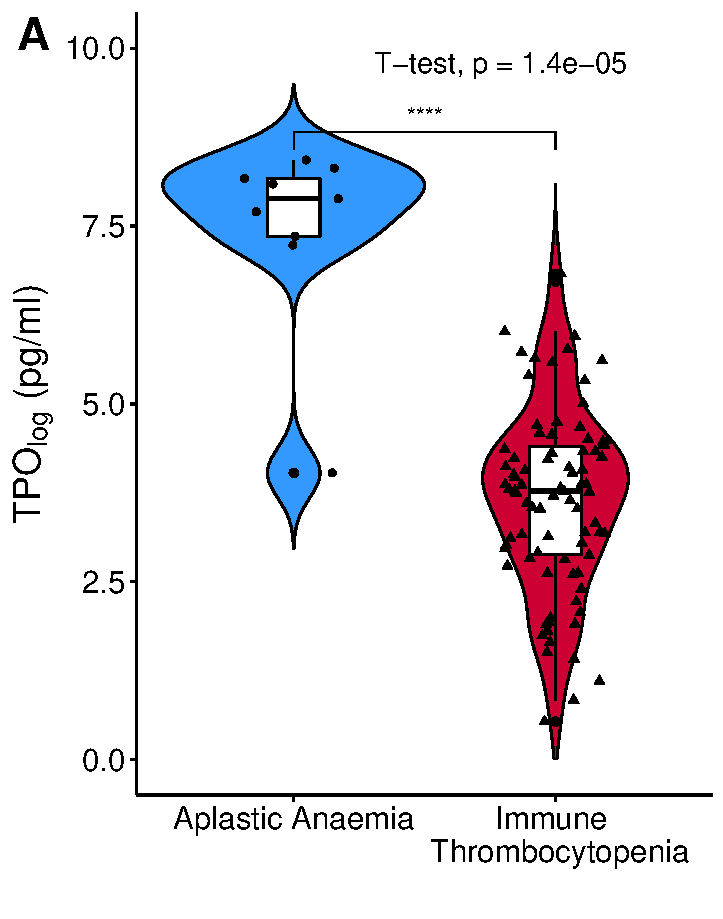
\includegraphics[width=0.29\linewidth]{fig/AA_vs_ITP_2.pdf}}}%
    \qquad
    {{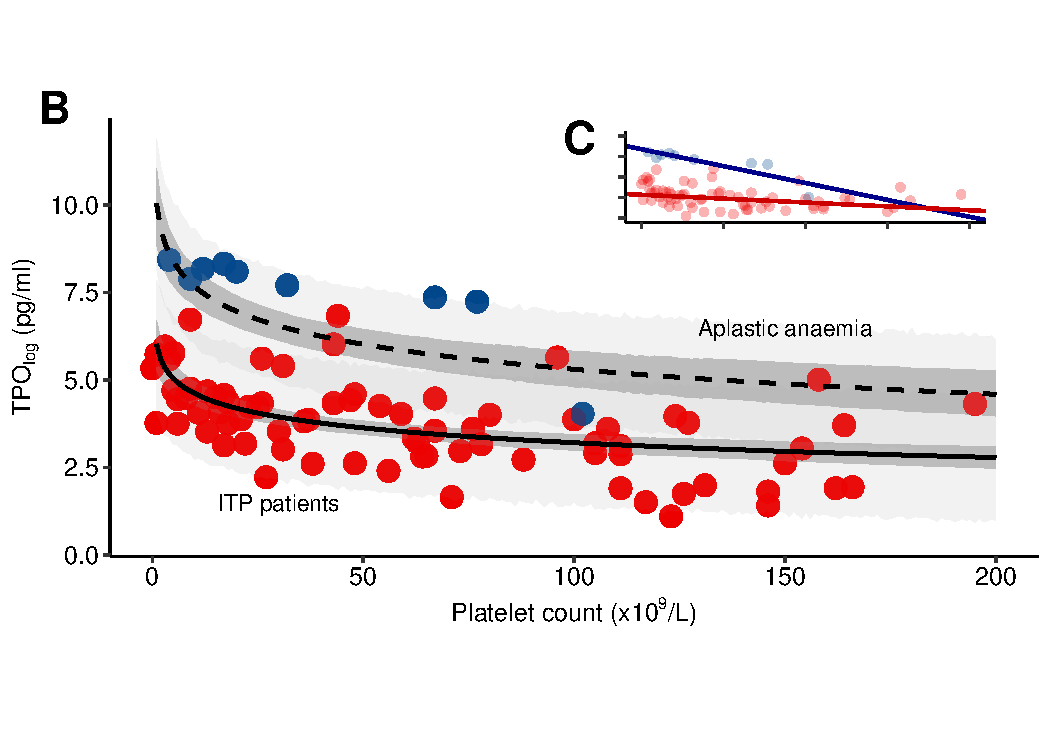
\includegraphics[width=0.67\linewidth]{fig/bayes_model2.pdf}}}%
    \caption{\textbf{A}: TPO levels in patients with Aplastic anaemia (AA) versus ITP. Of note there are 3 outliers within the AA group with lower TPO and platelet counts. These patients had received tacrolimus therapy prior to the study. \textbf{B}: log(TPO) levels versus platelet counts in ITP (red) and AA (blue). The graph shows the \textit{\textbf{MAP}} estimates \emph{(black lines)} and \textit{\textbf{90\% BIC interval}} (dark grey) as well as \textit{\textbf{total sampling area}} (light grey). \textbf{C}: Shows the same graph as in B, except the a linear regression model is fitted. This gives a visual demonstration of the difference between these two regression methods.}%
    \label{fig:example}%
\end{figure}


%\begin{figure}
%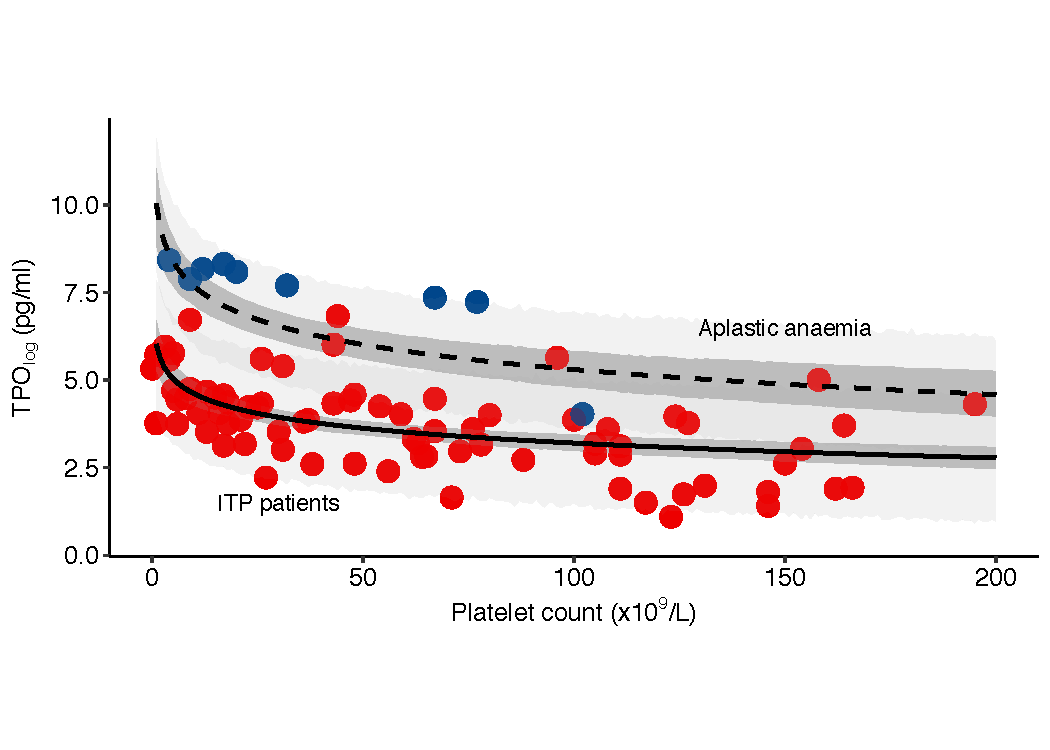
\includegraphics[width=0.8\linewidth]{fig/Bayes_model.pdf}
%\caption{Figure caption}
%\end{figure}


%\begin{alertblock}{Important Result}



%\end{alertblock} 

%----------------------------------------------------------------------------------------

\begin{columns}[t,totalwidth=\twocolwid] % Split up the two columns wide column again

\begin{column}{\onecolwid} % The first column within column 2 (column 2.1)

%----------------------------------------------------------------------------------------
%	MATHEMATICAL SECTION
%----------------------------------------------------------------------------------------

%\begin{block}{Methods...(continued)}
%\paragraph{} We used log-normalised TPO and platelet counts in a bayesian regression model;
%\begin{align}
%    \log(TPO) \thicksim \text{Norm}(\mu, \sigma) \\
%    \mu = \alpha + \beta\times \log(platelet) \\
%    \alpha \thicksim\ \text{Norm}(0.01, 10) \\
%    \beta \thicksim\ \text{Norm}(0.01, 10) \\
%    \sigma \thicksim \text{Uniform}(-1, 1)
%\end{align}
%\paragraph{} We used uninformative priors for the model (\textit{equation 3, 4, 5}) We used gibbs sampling with 100,000 iterations to calculate posterior distributions from which we derived \textbf{\textit{maximium a posteriori} (MAP)} estimates and 90\% Bayesian Confidence intervals (BCI) for a range of platelet counts (1 to 200$x10^9/L$).

%\end{block}
%----------------------------------------------------------------------------------------
\begin{block}{Results}

\paragraph{} In total 130 blood samples were collected from the 72 patients. 30 of the samples were excluded for failing to detect any TPO. All but 1 of these samples were from patients who had a second positive sample. In the ITP group, median TPO levels was 43pg/ml (range 1.7 - 923.4pg/ml) with a median platelet count of 63$\times 10^9/L$ (range 3 - 328$\times 10^9/L$). 20\% of this group were in remission at the time of sampling (platelet count >100$\times 10^9/L$) . In the aplastic anaemia cohort there were 9 samples in total with a median TPO of 1887.6pg/ml (range 9.4-4572.5pg/ml) and a median platelet count of 20$\times 10^9/L$ (range 4 - 102$\times 10^9/L$). The higher platelet counts (\>35$\times 10^9/L$) in this aplastic group were from patients on tacrolimus therapy (n= 3) (\textit{\textbf{FIGURE 1A}}). 

\vspace{30pt}

\paragraph{} The bayesian model used in this study identified a non-linear relationship between platelet counts and TPO levels in both ITP and aplastic anaemia (AA) patients (\textbf{\emph{FIGURE 1B}}), with consistently lower TPO levels in ITP. 

\end{block}



\end{column} % End of column 2.1

\begin{column}{\onecolwid} % The second column within column 2 (column 2.2)

%----------------------------------------------------------------------------------------
%	RESULTS
%----------------------------------------------------------------------------------------
\begin{block}{Results...(continued)}
\begin{figure}[H]
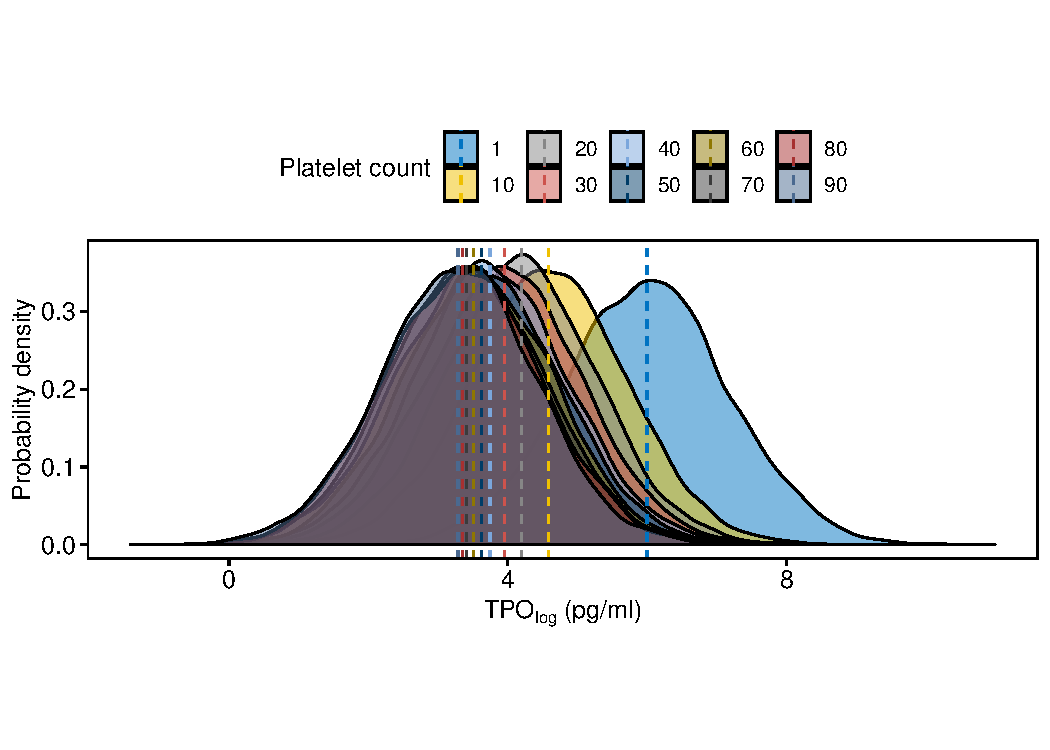
\includegraphics[width=0.8\linewidth]{fig/Probability_density.pdf}
\caption{Predicted \textit{maximium a posteriori} (MAP) distributions at various platelet counts ranging from 1 to 90$\times 10^9/L$. This shows that once platelet counts rise above 10$\times 10^9/L$ the probability distributions of TPO increasingly overlap}
\end{figure}

At any given platelet count, MAP estimates for TPO in our ITP cohort were approximately a tenth of that for patients with aplastic anaemia. The inferred distributions and MAP estimates from the ITP bayesian model can be seen in \textbf{\emph{FIGURE 2}}.


% At a platelet count of 1 the MAP TPO estimate in ITP was 410pg/ml (BCI; 200-804pg/ml). This declined sharply to 100pg/ml as platelet counts increased to 10$\times 10^9/L$. The decline in TPO became increasingly shallow as platelet counts increased further, and at 100$\times 10^9/L$ it was 24pg/ml (BCI 18-29 pg/ml). In contrast, MAP TPO estimates in the aplastic anaemia group were >10000pg/ml at a platelet count of $\times 10^9/L$ and 221pg/ml (BIC 112 to 828pg/ml) at 100$\times 10^9/L$. This is approaching the normal range for a healthy individual (mean 120pg/ml, range 80 - 230pg/ml).





%\begin{figure}
%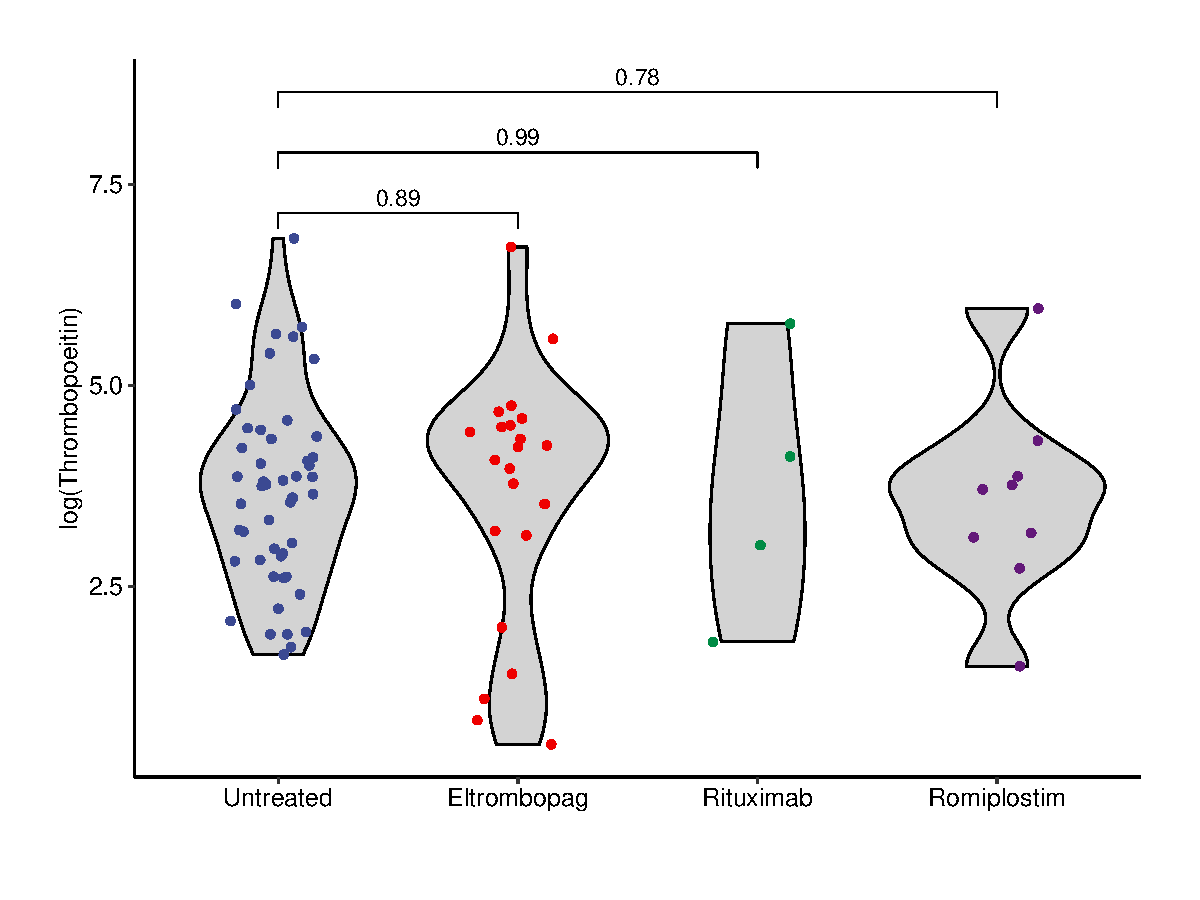
\includegraphics[width=1\linewidth]{fig/Static_diff_itp_only.pdf}
%\caption{Figure caption}
%\end{figure}

\end{block}

%----------------------------------------------------------------------------------------

\end{column} % End of column 2.2

\end{columns} % End of the split of column 2

\end{column} % End of the second column

\begin{column}{\sepwid}\end{column} % Empty spacer column

\begin{column}{\onecolwid} % The third column

%----------------------------------------------------------------------------------------
%	CONCLUSION
%----------------------------------------------------------------------------------------

\begin{block}{Results...(continued)}
\paragraph{} 
%\paragraph{} When compared to other regression models, the bayesian method had the lowest '\emph{deviance information criterion}' (DIC) score at 253.89 when compared to linear and polynomial models. The DIC score for the linear regression model (figure 1c) was 265.52. 
\begin{figure}
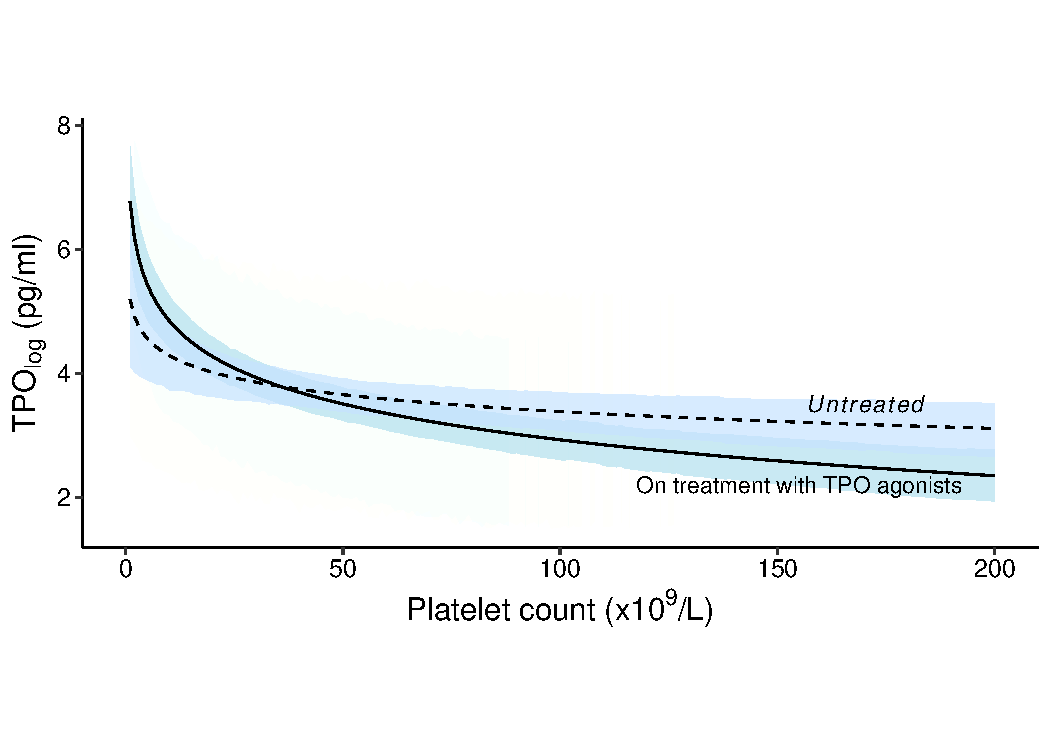
\includegraphics[width=0.8\linewidth]{fig/treatment1.pdf}
\caption{Fitted regression curve from models performed with patients on TPO agonists (Eltrombopag or Romiplostim) and those patients not on therapy at the time of blood sampling}
\end{figure}


\paragraph{} A quarter (25\%, n = 17) of the ITP patients recruited to the study were treated with TPO agonists and 60\% (n = 40) of the cohort were not on any treatment at the time of sampling. TPO levels were on average higher in untreated patients only when  platelet counts were >50$\times 10^9/L$. The opposite was the case at lower platelet counts (\textbf{\emph{FIGURE 3}}).  

\end{block}


\begin{block}{Conclusion}

\paragraph{} This study demonstrates that TPO levels in ITP are consistently lower than aplastic anaemia, irrespective of platelet count but the relationship between platelet counts and TPO is non-linear. These findings are consistent with megakaryocyte mass having a dominant influence on TPO levels. However, platelets also seem to exert some influence on circulating TPO levels but only when the platelet count falls below 40-50$\times10^9/L$. The cross-over of model estimates observed in \textbf{\emph{FIGURE 3}} is hard to explain. One hypothesis is that TPO agonists both increase the megakaryocyte pool causing greater TPO sponging, but also compete for the MPL-receptor thus causing a small rise in circulating TPO. The relative influence of these two processes on TPO levels may change as the platelet count varies.  

\end{block}

%----------------------------------------------------------------------------------------
%	ADDITIONAL INFORMATION
%----------------------------------------------------------------------------------------

%\begin{block}{Additional Information}

%Maecenas ultricies feugiat velit non mattis. Fusce tempus arcu id ligula varius dictum. 
%\begin{itemize}
%\item Curabitur pellentesque dignissim
%\item Eu facilisis est tempus quis
%\item Duis porta consequat lorem
%\end{itemize}

%\end{block}

%----------------------------------------------------------------------------------------
%	REFERENCES
%----------------------------------------------------------------------------------------

\begin{block}{References}

%\nocite{*} % Insert publications even if they are not cited in the poster
\small{\bibliographystyle{ieeetr}
\bibliography{sample}\vspace{0.2in}}

\end{block}

%----------------------------------------------------------------------------------------
%	ACKNOWLEDGEMENTS
%----------------------------------------------------------------------------------------

\setbeamercolor{block title}{fg=red,bg=white} % Change the block title color

%\begin{block}{Acknowledgements}

%\small{\rmfamily{This work is entirely of my own}} \\

%\end{block}

%----------------------------------------------------------------------------------------
%	CONTACT INFORMATION
%----------------------------------------------------------------------------------------

\setbeamercolor{block alerted title}{fg=black,bg=norange} % Change the alert block title colors
\setbeamercolor{block alerted body}{fg=black,bg=white} % Change the alert block body colors

%\begin{alertblock}{Contact Information}

%\begin{itemize}
%\item Web: \href{http://www.university.edu/smithlab}{http://www.university.edu/smithlab}
%\item Email: \href{}{george.adams2@imperial.ac.uk}
%\end{itemize}

%\end{alertblock}

%\begin{center}
%\begin{tabular}{ccc}
%
\includegraphics[width=0.4\linewidth]{logo.png} & \hfill & %
\includegraphics[width=0.4\linewidth]{logo.png}
%\end{tabular}
%\end{center}

%----------------------------------------------------------------------------------------

\end{column} % End of the third column

\end{columns} % End of all the columns in the poster

\end{frame} % End of the enclosing frame

\end{document}
